\documentclass{article}
\usepackage[legalpaper, portrait, margin=0.5in]{geometry}
\usepackage{tikz}
\usetikzlibrary{arrows.meta, positioning}
\title{CSC226 Exercise 9}
\author{Dryden Bryson}
\date{\today}

\begin{document}

\maketitle
\newpage
Consider the following graph $G$:\\
\begin{center}
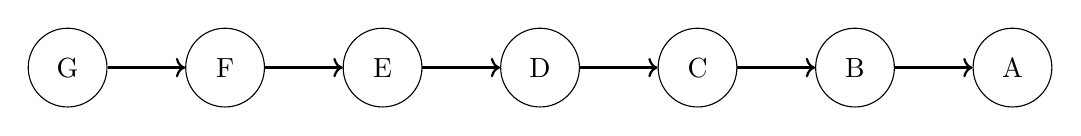
\begin{tikzpicture}[
    node distance=2cm,
    every node/.style={circle, draw, minimum size=1cm},
    arrow/.style={->, thick}
]

\node (G) {G};
\node (F) [right of=G] {F};
\node (E) [right of=F] {E};
\node (D) [right of=E] {D};
\node (C) [right of=D] {C};
\node (B) [right of=C] {B};
\node (A) [right of=B] {A};

\draw[arrow] (G) -- (F);
\draw[arrow] (F) -- (E);
\draw[arrow] (E) -- (D);
\draw[arrow] (D) -- (C);
\draw[arrow] (C) -- (B);
\draw[arrow] (B) -- (A);
\end{tikzpicture}
\end{center}
Now let us observe the following iterations of Floyd-Wartshall-Roy algorithm on $G$ and specifically the entrance on the distance matrix GB, here the dotted edges represent the edges of the graph and the red edges represent the known paths, for simplicities sake and sake of my sanity writing this latex document, we will assume all edges have weight 1 and intermediary paths will not be displyed, I.E if we have discovered a path from E to B, the path D to B will not be displayed:\\
\begin{itemize}
    \item $k=0$ (Initialization):\\[6pt]
    \begin{minipage}[c]{0.4\textwidth}
    \begin{tabular}{c|c|c|c|c|c|c|c} 
     &       A  & B         & C         & D         & E         & F         & G         \\
        \hline
   A &       0  & $\infty$  & $\infty$  &$ \infty$  & $\infty$  & $\infty$  & $\infty$  \\
        \hline
   B &       1  &        0  & $\infty$  & $\infty$  & $\infty$  & $\infty$  & $\infty$  \\
        \hline
   C & $\infty$ &       1  &        0   & $\infty$  & $\infty$  & $\infty$  & $\infty$  \\
        \hline
   D & $\infty$ & $\infty$ &        1   &        0  & $\infty$  & $\infty$  & $\infty$  \\
        \hline
   E & $\infty$ & $\infty$ & $\infty$   &         1 &         0 & $\infty$  & $\infty$  \\
        \hline
   F & $\infty$ & $\infty$ & $\infty$   & $\infty$  &         1 &        0  & $\infty$  \\
        \hline
   G & $\infty$ & $\infty$ & $\infty$   & $\infty$  & $\infty$  &        1  &  0        \\
    \end{tabular}
    \end{minipage}%
    \begin{minipage}[c]{0.6\textwidth}
    \centering
    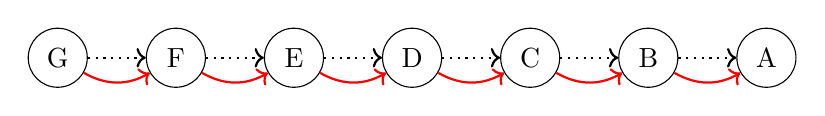
\begin{tikzpicture}[
        node distance=1.5cm,
        every node/.style={circle, draw, minimum size=0.75cm},
        arrow/.style={->, thick}
    ]

    \tikzset{
    arrow/.style={->, thick, dotted},
    known/.style={->, thick, red, bend left=30}
}

    \node (G) {G};
    \node (F) [right of=G] {F};
    \node (E) [right of=F] {E};
    \node (D) [right of=E] {D};
    \node (C) [right of=D] {C};
    \node (B) [right of=C] {B};
    \node (A) [right of=B] {A};

    \draw[arrow] (G) -- (F);
    \draw[arrow] (F) -- (E);
    \draw[arrow] (E) -- (D);
    \draw[arrow] (D) -- (C);
    \draw[arrow] (C) -- (B);
    \draw[arrow] (B) -- (A);

    \draw[known] (G) to[bend right=30] (F);
    \draw[known] (F) to[bend right=30] (E);
    \draw[known] (E) to[bend right=30] (D);
    \draw[known] (D) to[bend right=30] (C);
    \draw[known] (C) to[bend right=30] (B);
    \draw[known] (B) to[bend right=30] (A);
    \end{tikzpicture}
    \end{minipage}

    \item $k=1$ (Node A is intermediary):\\[6pt]
    \begin{minipage}[c]{0.4\textwidth}
    \begin{tabular}{c|c|c|c|c|c|c|c} 
     &       A  & B         & C         & D         & E         & F         & G         \\
        \hline
   A &       0  & $\infty$  & $\infty$  &$ \infty$  & $\infty$  & $\infty$  & $\infty$  \\
        \hline
   B &       1  &        0  & $\infty$  & $\infty$  & $\infty$  & $\infty$  & $\infty$  \\
        \hline
   C & $\infty$ &       1  &        0   & $\infty$  & $\infty$  & $\infty$  & $\infty$  \\
        \hline
   D & $\infty$ & $\infty$ &        1   &        0  & $\infty$  & $\infty$  & $\infty$  \\
        \hline
   E & $\infty$ & $\infty$ & $\infty$   &         1 &         0 & $\infty$  & $\infty$  \\
        \hline
   F & $\infty$ & $\infty$ & $\infty$   & $\infty$  &         1 &        0  & $\infty$  \\
        \hline
   G & $\infty$ & $\infty$ & $\infty$   & $\infty$  & $\infty$  &        1  &  0        \\
    \end{tabular}
    \end{minipage}%
    \begin{minipage}[c]{0.6\textwidth}
    \centering
    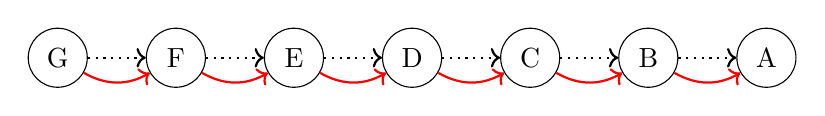
\begin{tikzpicture}[
        node distance=1.5cm,
        every node/.style={circle, draw, minimum size=0.75cm},
        arrow/.style={->, thick}
    ]

    \tikzset{
    arrow/.style={->, thick, dotted},
    known/.style={->, thick, red, bend left=30}
}

    \node (G) {G};
    \node (F) [right of=G] {F};
    \node (E) [right of=F] {E};
    \node (D) [right of=E] {D};
    \node (C) [right of=D] {C};
    \node (B) [right of=C] {B};
    \node (A) [right of=B] {A};

    \draw[arrow] (G) -- (F);
    \draw[arrow] (F) -- (E);
    \draw[arrow] (E) -- (D);
    \draw[arrow] (D) -- (C);
    \draw[arrow] (C) -- (B);
    \draw[arrow] (B) -- (A);

    \draw[known] (G) to[bend right=30] (F);
    \draw[known] (F) to[bend right=30] (E);
    \draw[known] (E) to[bend right=30] (D);
    \draw[known] (D) to[bend right=30] (C);
    \draw[known] (C) to[bend right=30] (B);
    \draw[known] (B) to[bend right=30] (A);
    \end{tikzpicture}
    \end{minipage}\\
    No new edges discovered as intermediary edge A has no outgoing edges

        \item $k=2$ (Node B is intermediary):\\[6pt]
    \begin{minipage}[c]{0.4\textwidth}
    \begin{tabular}{c|c|c|c|c|c|c|c} 
     &       A  & B         & C         & D         & E         & F         & G         \\
        \hline
   A &       0  & $\infty$  & $\infty$  &$ \infty$  & $\infty$  & $\infty$  & $\infty$  \\
        \hline
   B &       1  &        0  & $\infty$  & $\infty$  & $\infty$  & $\infty$  & $\infty$  \\
        \hline
   C & 2 &       1  &        0   & $\infty$  & $\infty$  & $\infty$  & $\infty$  \\
        \hline
   D & $\infty$ & $\infty$ &        1   &        0  & $\infty$  & $\infty$  & $\infty$  \\
        \hline
   E & $\infty$ & $\infty$ & $\infty$   &         1 &         0 & $\infty$  & $\infty$  \\
        \hline
   F & $\infty$ & $\infty$ & $\infty$   & $\infty$  &         1 &        0  & $\infty$  \\
        \hline
   G & $\infty$ & $\infty$ & $\infty$   & $\infty$  & $\infty$  &        1  &  0        \\
    \end{tabular}
    \end{minipage}%
    \begin{minipage}[c]{0.6\textwidth}
    \centering
    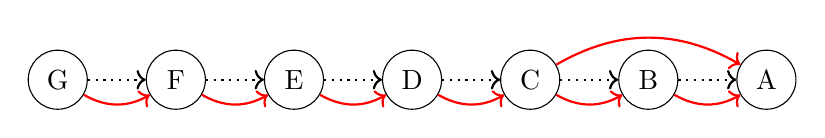
\begin{tikzpicture}[
        node distance=1.5cm,
        every node/.style={circle, draw, minimum size=0.75cm},
        arrow/.style={->, thick}
    ]

    \tikzset{
    arrow/.style={->, thick, dotted},
    known/.style={->, thick, red, bend left=30}
}

    \node (G) {G};
    \node (F) [right of=G] {F};
    \node (E) [right of=F] {E};
    \node (D) [right of=E] {D};
    \node (C) [right of=D] {C};
    \node (B) [right of=C] {B};
    \node (A) [right of=B] {A};

    \draw[arrow] (G) -- (F);
    \draw[arrow] (F) -- (E);
    \draw[arrow] (E) -- (D);
    \draw[arrow] (D) -- (C);
    \draw[arrow] (C) -- (B);
    \draw[arrow] (B) -- (A);

    \draw[known] (G) to[bend right=30] (F);
    \draw[known] (F) to[bend right=30] (E);
    \draw[known] (E) to[bend right=30] (D);
    \draw[known] (D) to[bend right=30] (C);
    \draw[known] (C) to[bend right=30] (B);
    \draw[known] (B) to[bend right=30] (A);

    \draw[known] (C) to[bend left=30] (A);
    \end{tikzpicture}
    \end{minipage}\\
    Path from C to A is discovered through intermediary edge B

    \item $k=3$ (Node C is intermediary):\\[6pt]
    \begin{minipage}[c]{0.4\textwidth}
    \begin{tabular}{c|c|c|c|c|c|c|c} 
     &       A  & B         & C         & D         & E         & F         & G         \\
        \hline
   A &       0  & $\infty$  & $\infty$  &$ \infty$  & $\infty$  & $\infty$  & $\infty$  \\
        \hline
   B &       1  &        0  & $\infty$  & $\infty$  & $\infty$  & $\infty$  & $\infty$  \\
        \hline
   C & 2 &       1  &        0   & $\infty$  & $\infty$  & $\infty$  & $\infty$  \\
        \hline
   D & 3 & 2 &        1   &        0  & $\infty$  & $\infty$  & $\infty$  \\
        \hline
   E & $\infty$ & $\infty$ & $\infty$   &         1 &         0 & $\infty$  & $\infty$  \\
        \hline
   F & $\infty$ & $\infty$ & $\infty$   & $\infty$  &         1 &        0  & $\infty$  \\
        \hline
   G & $\infty$ & $\infty$ & $\infty$   & $\infty$  & $\infty$  &        1  &  0        \\
    \end{tabular}
    \end{minipage}%
    \begin{minipage}[c]{0.6\textwidth}
    \centering
    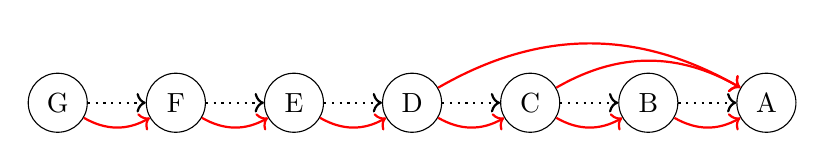
\begin{tikzpicture}[
        node distance=1.5cm,
        every node/.style={circle, draw, minimum size=0.75cm},
        arrow/.style={->, thick}
    ]

    \tikzset{
    arrow/.style={->, thick, dotted},
    known/.style={->, thick, red, bend left=30}
}

    \node (G) {G};
    \node (F) [right of=G] {F};
    \node (E) [right of=F] {E};
    \node (D) [right of=E] {D};
    \node (C) [right of=D] {C};
    \node (B) [right of=C] {B};
    \node (A) [right of=B] {A};

    \draw[arrow] (G) -- (F);
    \draw[arrow] (F) -- (E);
    \draw[arrow] (E) -- (D);
    \draw[arrow] (D) -- (C);
    \draw[arrow] (C) -- (B);
    \draw[arrow] (B) -- (A);

    \draw[known] (G) to[bend right=30] (F);
    \draw[known] (F) to[bend right=30] (E);
    \draw[known] (E) to[bend right=30] (D);
    \draw[known] (D) to[bend right=30] (C);
    \draw[known] (C) to[bend right=30] (B);
    \draw[known] (B) to[bend right=30] (A);

    \draw[known] (C) to[bend left=30] (A);
    \draw[known] (D) to[bend left=30] (A);
    \end{tikzpicture}
    \end{minipage}\\
    Path from D to A is discovered through intermediary node C which has a path to A

    \item $k=4$ (Node D is intermediary):\\[6pt]
    \begin{minipage}[c]{0.4\textwidth}
    \begin{tabular}{c|c|c|c|c|c|c|c} 
     &       A  & B         & C         & D         & E         & F         & G         \\
        \hline
   A &       0  & $\infty$  & $\infty$  &$ \infty$  & $\infty$  & $\infty$  & $\infty$  \\
        \hline
   B &       1  &        0  & $\infty$  & $\infty$  & $\infty$  & $\infty$  & $\infty$  \\
        \hline
   C & 2 &       1  &        0   & $\infty$  & $\infty$  & $\infty$  & $\infty$  \\
        \hline
   D & 3 & 2 &        1   &        0  & $\infty$  & $\infty$  & $\infty$  \\
        \hline
   E & 4 & 3 & 2   &         1 &         0 & $\infty$  & $\infty$  \\
        \hline
   F & $\infty$ & $\infty$ & $\infty$   & $\infty$  &         1 &        0  & $\infty$  \\
        \hline
   G & $\infty$ & $\infty$ & $\infty$   & $\infty$  & $\infty$  &        1  &  0        \\
    \end{tabular}
    \end{minipage}%
    \begin{minipage}[c]{0.6\textwidth}
    \centering
    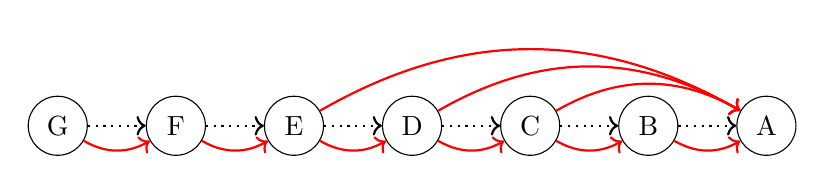
\begin{tikzpicture}[
        node distance=1.5cm,
        every node/.style={circle, draw, minimum size=0.75cm},
        arrow/.style={->, thick}
    ]

    \tikzset{
    arrow/.style={->, thick, dotted},
    known/.style={->, thick, red, bend left=30}
}

    \node (G) {G};
    \node (F) [right of=G] {F};
    \node (E) [right of=F] {E};
    \node (D) [right of=E] {D};
    \node (C) [right of=D] {C};
    \node (B) [right of=C] {B};
    \node (A) [right of=B] {A};

    \draw[arrow] (G) -- (F);
    \draw[arrow] (F) -- (E);
    \draw[arrow] (E) -- (D);
    \draw[arrow] (D) -- (C);
    \draw[arrow] (C) -- (B);
    \draw[arrow] (B) -- (A);

    \draw[known] (G) to[bend right=30] (F);
    \draw[known] (F) to[bend right=30] (E);
    \draw[known] (E) to[bend right=30] (D);
    \draw[known] (D) to[bend right=30] (C);
    \draw[known] (C) to[bend right=30] (B);
    \draw[known] (B) to[bend right=30] (A);

    \draw[known] (C) to[bend left=30] (A);
    \draw[known] (D) to[bend left=30] (A);
    \draw[known] (E) to[bend left=30] (A);
    \end{tikzpicture}
    \end{minipage}\\
    Path from E to A is discovered through intermediary node D which has a path to A

        \item $k=5$ (Node E is intermediary):\\[6pt]
    \begin{minipage}[c]{0.4\textwidth}
    \begin{tabular}{c|c|c|c|c|c|c|c} 
     &       A  & B         & C         & D         & E         & F         & G         \\
        \hline
   A &       0  & $\infty$  & $\infty$  &$ \infty$  & $\infty$  & $\infty$  & $\infty$  \\
        \hline
   B &       1  &        0  & $\infty$  & $\infty$  & $\infty$  & $\infty$  & $\infty$  \\
        \hline
   C & 2 &       1  &        0   & $\infty$  & $\infty$  & $\infty$  & $\infty$  \\
        \hline
   D & 3 & 2 &        1   &        0  & $\infty$  & $\infty$  & $\infty$  \\
        \hline
   E & 4 & 3 & 2   &         1 &         0 & $\infty$  & $\infty$  \\
        \hline
   F & 5 & 4 & 3   & 2   &         1 &        0  & $\infty$  \\
        \hline
   G & $\infty$ & $\infty$ & $\infty$   & $\infty$  & $\infty$  &        1  &  0        \\
    \end{tabular}
    \end{minipage}%
    \begin{minipage}[c]{0.6\textwidth}
    \centering
    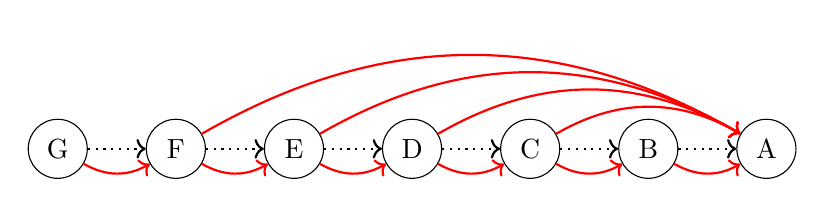
\begin{tikzpicture}[
        node distance=1.5cm,
        every node/.style={circle, draw, minimum size=0.75cm},
        arrow/.style={->, thick}
    ]

    \tikzset{
    arrow/.style={->, thick, dotted},
    known/.style={->, thick, red, bend left=30}
}

    \node (G) {G};
    \node (F) [right of=G] {F};
    \node (E) [right of=F] {E};
    \node (D) [right of=E] {D};
    \node (C) [right of=D] {C};
    \node (B) [right of=C] {B};
    \node (A) [right of=B] {A};

    \draw[arrow] (G) -- (F);
    \draw[arrow] (F) -- (E);
    \draw[arrow] (E) -- (D);
    \draw[arrow] (D) -- (C);
    \draw[arrow] (C) -- (B);
    \draw[arrow] (B) -- (A);

    \draw[known] (G) to[bend right=30] (F);
    \draw[known] (F) to[bend right=30] (E);
    \draw[known] (E) to[bend right=30] (D);
    \draw[known] (D) to[bend right=30] (C);
    \draw[known] (C) to[bend right=30] (B);
    \draw[known] (B) to[bend right=30] (A);

    \draw[known] (C) to[bend left=30] (A);
    \draw[known] (D) to[bend left=30] (A);
    \draw[known] (E) to[bend left=30] (A);
    \draw[known] (F) to[bend left=30] (A);
    \end{tikzpicture}
    \end{minipage}\\
    Path from F to A is discovered through intermediary node E which has a path to A
\end{itemize}

As we can see exluding the initialization that after 5 iterations, any non direct outgoing path fron G has not been discovered including the path from G to B, which contains 5 edges and thus disproving the given claim.

    


\end{document}
